\documentclass[a4paper,11pt]{article}

\usepackage[utf8]{inputenc} % Unicode support (Umlauts etc.)
\usepackage[ngerman]{babel} % Change hyphenation rules
\usepackage{ziffer} % , können in Zahlen verwendet werden ohne Formatierung kaputt zu machen
\usepackage[top=30mm,right=20mm,bottom=15mm,left=25mm,includefoot,headheight=28pt]{geometry} % Seitenränder

\usepackage{lmodern,textcomp} % The package supports the Text Companion fonts, which provide many text symbols (benötigt für €)
\usepackage[fleqn]{amsmath} % Formatierte Gleichungen
\usepackage{graphicx} % Grafiken
\usepackage{xcolor} % Farbe in Text
\usepackage{fancyhdr} % Seitenstil mit Kopfzeile etc.

\usepackage{cases} % FAllunterscheidungen mathematisch uebereinander

\pagestyle{fancy}
\fancyhf{}
\lhead{Lösung \\Übungsblatt 4}
\rhead{Gruppe 3 \\Nils \textbf{Hodys}, Sascha \textbf{Majewsky}}
\rfoot{Seite \thepage}

\setlength{\parindent}{0cm} % Keine Einrückung der 1. Zeile eines Absatzes

\begin{document}

\raggedright % Alles Linksbündig

\section*{Aufgabe 1}

\subsection*{Entscheidungsvariablen} 
\subsubsection*{Kontinuierliche Variablen}
$x_{s}$: ha Ackerfläche pro Anbauperiode zur Produktion von Schnaps \\
$x_{b}$: ha Ackerfläche pro Anbauperiode zur Produktion von Bier \\
$x_{w}$: ha Ackerfläche pro Anbauperiode zur Produktion von Wein \\
\bigbreak

\subsubsection*{Binärvariablen}
\begin{align*}
y_s &= \begin{cases}
    1, & \text{wenn Schnapsproduktion mit Fixkosten 3900 GE} \\
    0, & \text{sonst keine Schnapsproduktion mit keinen Fixkosten}
\end{cases} \\
y_b &= \begin{cases}
    1, & \text{wenn Bierproduktion mit Fixkosten 4900 GE} \\
    0, & \text{sonst keine Bierproduktion mit keinen Fixkosten}
\end{cases} \\
y_w &= \begin{cases}
    1, & \text{wenn Weinproduktion mit Fixkosten 6600 GE} \\
    0, & \text{sonst keine Weinproduktion mit keinen Fixkosten}
\end{cases}
\end{align*}

\subsection*{Modellierung}
Anmerkung: \\
Es gibt keine Mindestbestellmengen an Ackerfläche pro Jahr pro Produkt und daher sind in Bezug dessen keine Schwellenwerte zu beachten. \\
Die Aufgabenstellung verlangt nicht, dass nur vollständige Fässer abgefüllt werden können.

\bigbreak
Zielfunktion: \\
Zielfunktion mit Gewinnmaximierung abzüglich Fixkosten. Koeffizienten von $x_n$ in GE / ha.

\begin{align*}
    \text{max. } & z = 15000x_{s} + 27000x_{b} + 36000x_{w} - 3900y_{s} - 4900y_{b} - 6600y_{w}
\end{align*}
\begin{align*}
    \text{s.t. } & x_{s} + x_{b} + x_{w} \le 100 && \text{Max. Gesamtanbaufläche 100 Hektar} \\
    & 60x_{s} + 60x_{b} + 48x_{w} \le 5200 && \text{Es stehen maximal 5200 50l-Fässer zur Verfügung} \\
    & x_{s} \le 60*y_{s} && \text{Max. 60ha für Schnaps u. Binärverknüpfung} \\
    & x_{b} \le 50*y_{b} && \text{Max. 50ha für Bier u. Binärverknüpfung} \\
    & x_{w} \le 60\frac{5}{12}*y_{w} && \text{Max $60\frac{5}{12}$ha für Wein u. Binärverknüpfung} \\
    & x_{s}, x_{b}, x_{w} \ge 0 && \text{Es kann keine negative Menge produziert werden} \\
    & y_{s}, y_{b}, y_{w} \in \{ 0,1 \} && \text{Definition der Binärvariablen} \\
\end{align*}

\subsection*{Lingo Solver}
\begin{centering}
	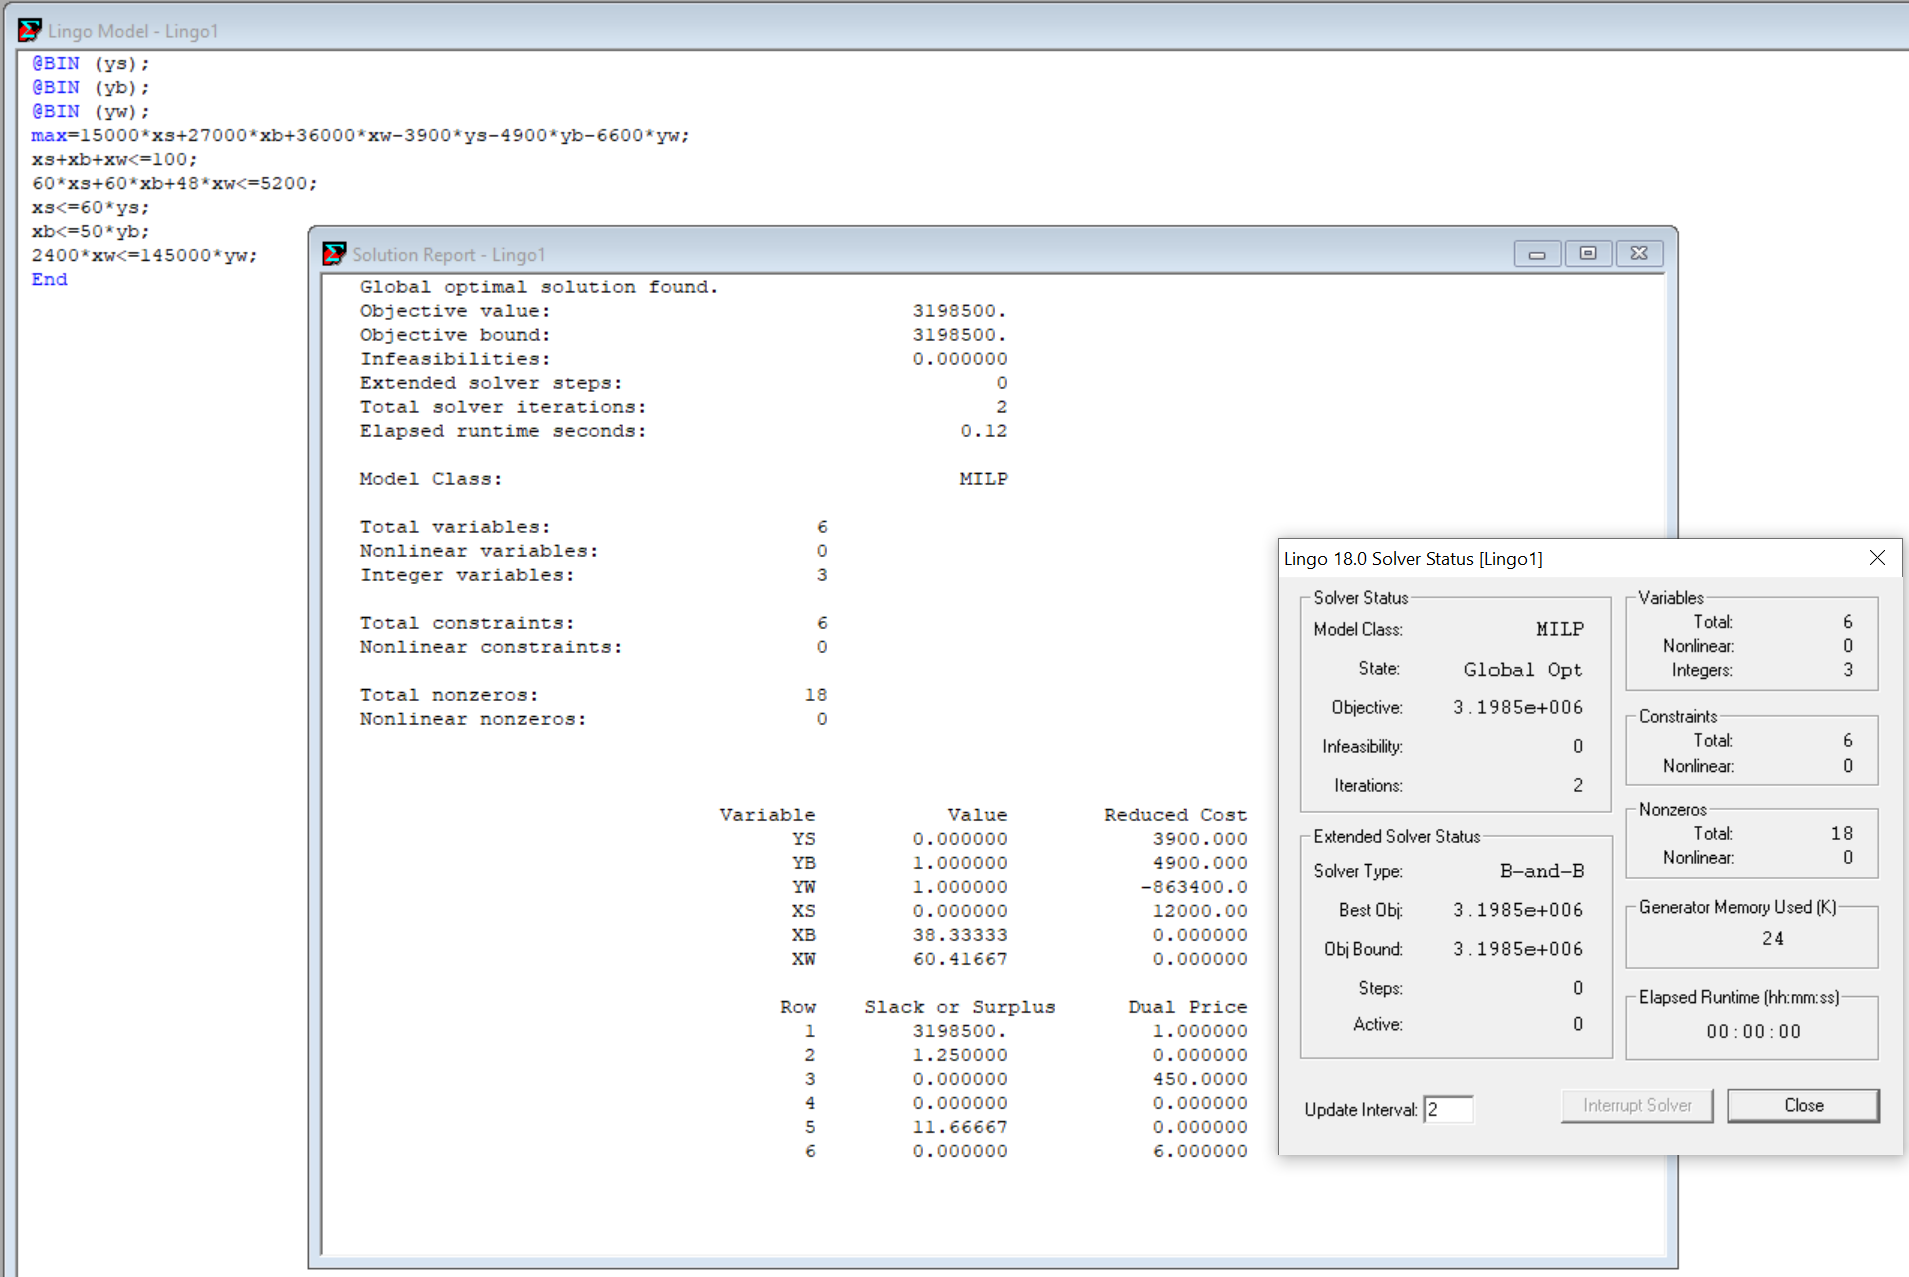
\includegraphics[width=1\linewidth]{src/blatt_4_aufgabe_1_loesung_solver.PNG}
\end{centering}

$\to$ \textbf{Getränkeherstellerberatung Optimalfall:} \\
\begin{itemize}
    \item Im Optimalfall wird pro Anbauperiode nur Bier und Wein angebaut. \\
    \item Dann verteilt sich die Bestellung des Ackers pro Anbauperiode auf 38,33333 ha Hopfen und 60,41667 ha Weintrauben. \\
    \item Es bleiben auf Grund der Restriktionen der Abfülling in 50l Fässer pro Anbauperiode 1,25 ha nutzbarer Ackerfläche übrig, welche privat oder für andere wirtschaftliche Geschäfte genutzt werden kann. Es bleiben keine Fässer mehr übrig.
\end{itemize}

\section*{Aufgabe 2}

\subsection*{Entscheidungsvariablen}
\subsubsection*{Kontinuierliche Variablen}
$x_{M}$: Anzurichtender Salat Mediterran in Portionen \\
$x_{L}$: Anzurichtender Salat Latin in Portionen \\
$x_{C}$: Anzurichtender Salat Classic in Portionen \\
\pagebreak

\subsubsection*{Binärvariablen}

\begin{align*}
y_M &= \begin{cases}
    1, & \text{wenn Anrichtung Salat M} \\
    0, & \text{wenn keine Anrichtung Salat M}
\end{cases} \\
y_L &= \begin{cases}
    1, & \text{wenn Anrichtung Salat L} \\
    0, & \text{wenn keine Anrichtung Salat L}
\end{cases} \\
y_C &= \begin{cases}
    1, & \text{wenn Anrichtung Salat C} \\
    0, & \text{wenn keine Anrichtung Salat C}
\end{cases}
\end{align*}

\subsection*{Modellierung}

Anmerkung: \\
\begin{itemize}
    \item Falls ein Salat angerichtet wird gibt es eine Mindestmenge (30), daher werden Schwellenwerte relevant \\
    \item Ein Schwellenwert ist entweder 0 oder Mindestmenge bis Höchstmenge \\
    \item Uns ist die Mindestmenge mit 30 Portionen bekannt, daher ist eine Ermittlung mittels Big-M durch Restriktionsbeziehungen nicht nötig
\end{itemize}
    \bigbreak
    Zielfunktion: \\
\begin{itemize}
    \item Zielfunktion mit Umsatzmaximierung und Binärverknüpfung
\end{itemize}

%\subsection*{LP}
\begin{align*}
    \text{max. } & z = 3,90x_{M} \cdot y_{M} + 4,30x_{L} \cdot y_{L} + 3,60x_{C} \cdot y_{C} \\
    \\
    \text{s.t. } & x_{M} + x_{L} + x_{C} \le 180 && \text{6 Mitarbeiter können täglich 30 Salate anrichten} \\
    & 300x_{M} + 200x_{L} + 250x_{C} \le 48000 && \text{Tomatenbestand Gramm} \\
    & 150x_{M} + 110x_{L} + 150x_{C} \le 25000 && \text{Paprikabestand Gramm} \\
    & 150x_{M} + 120x_{C} \le 19000 && \text{Gurkenbestand Gramm} \\
    & 200x_{L} \le 11000 && \text{Mangobestand Gramm} \\
    & 250x_{M} \le 8000 && \text{Rucolabestand Gramm} \\
    & 180x_{L} \le 6000 && \text{Avocadobestand Gramm} \\
    & 220x_{C} \le 12000 && \text{Kichererbsenbestand Gramm} \\
    & 40x_{M} + 35x_{L} \le 5000 && \text{Olivenölbestand ml} \\
    & 70x_{C} \le 5000 && \text{Fetabestand Gramm} \\
    & x_{M} \ge 30*y_{M} && \text{Salat M Binärverknüpfung} \\
    & x_{L} \ge 30*y_{L} && \text{Salat L Binärverknüpfung} \\
    & x_{C} \ge 30*y_{C} && \text{Salat C Binärverknüpfung} \\
    & x_{M}, x_{L}, x_{C} \ge 0 && \text{Es kann keine negative Menge angerichtet werden} \\
    & y_{M}, y_{L}, y_{C} \in \{ 0,1 \} && \text{Wertzuweisung Binärvariablen} \\
\end{align*}

\subsection*{Lösung laut Solver}
\begin{centering}
	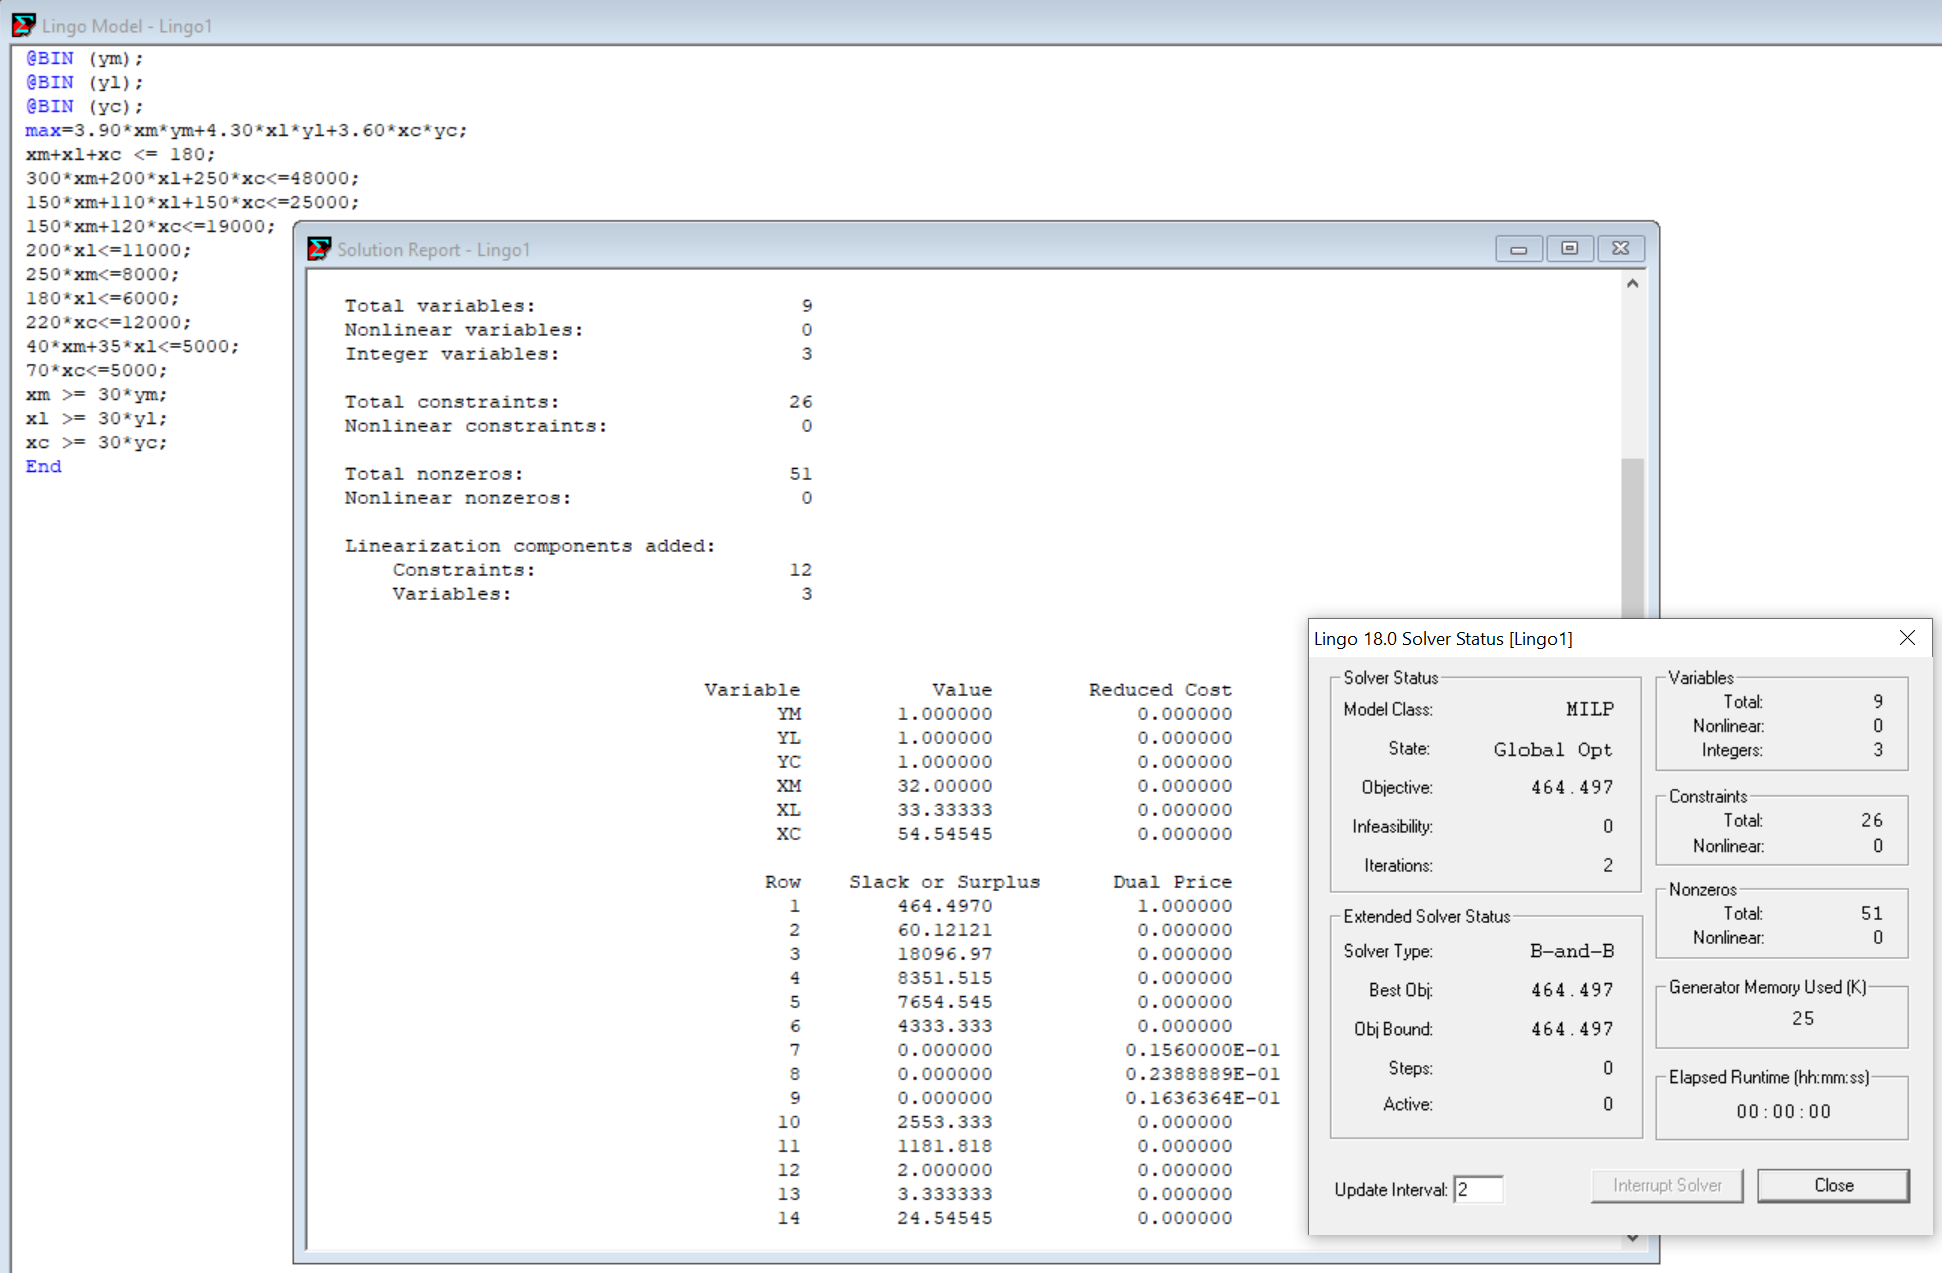
\includegraphics[width=1\linewidth]{src/blatt_4_aufgabe_2_loesung_solver.PNG}
\end{centering}

\subsection*{Ganzzahligkeit}
Aus der Aufgabe geht nicht hervor, ob nur vollständige Salate produziert werden können. Wenn angenommen werden soll, dass nur ganze Salate produziert werden können, muss die Restriktion der Ganzzahligkeit hinzugefügt werden. \newline

Die vorletzte Restriktion muss dann lauten:
\begin{align*}
x_{M}, x_{L}, x_{C} \ge 0, \text{integer}
\end{align*}

Zudem müssen die Variablen in Lingo mit \textit{@GIN} als Integer deklariert werden:

\begin{centering}
	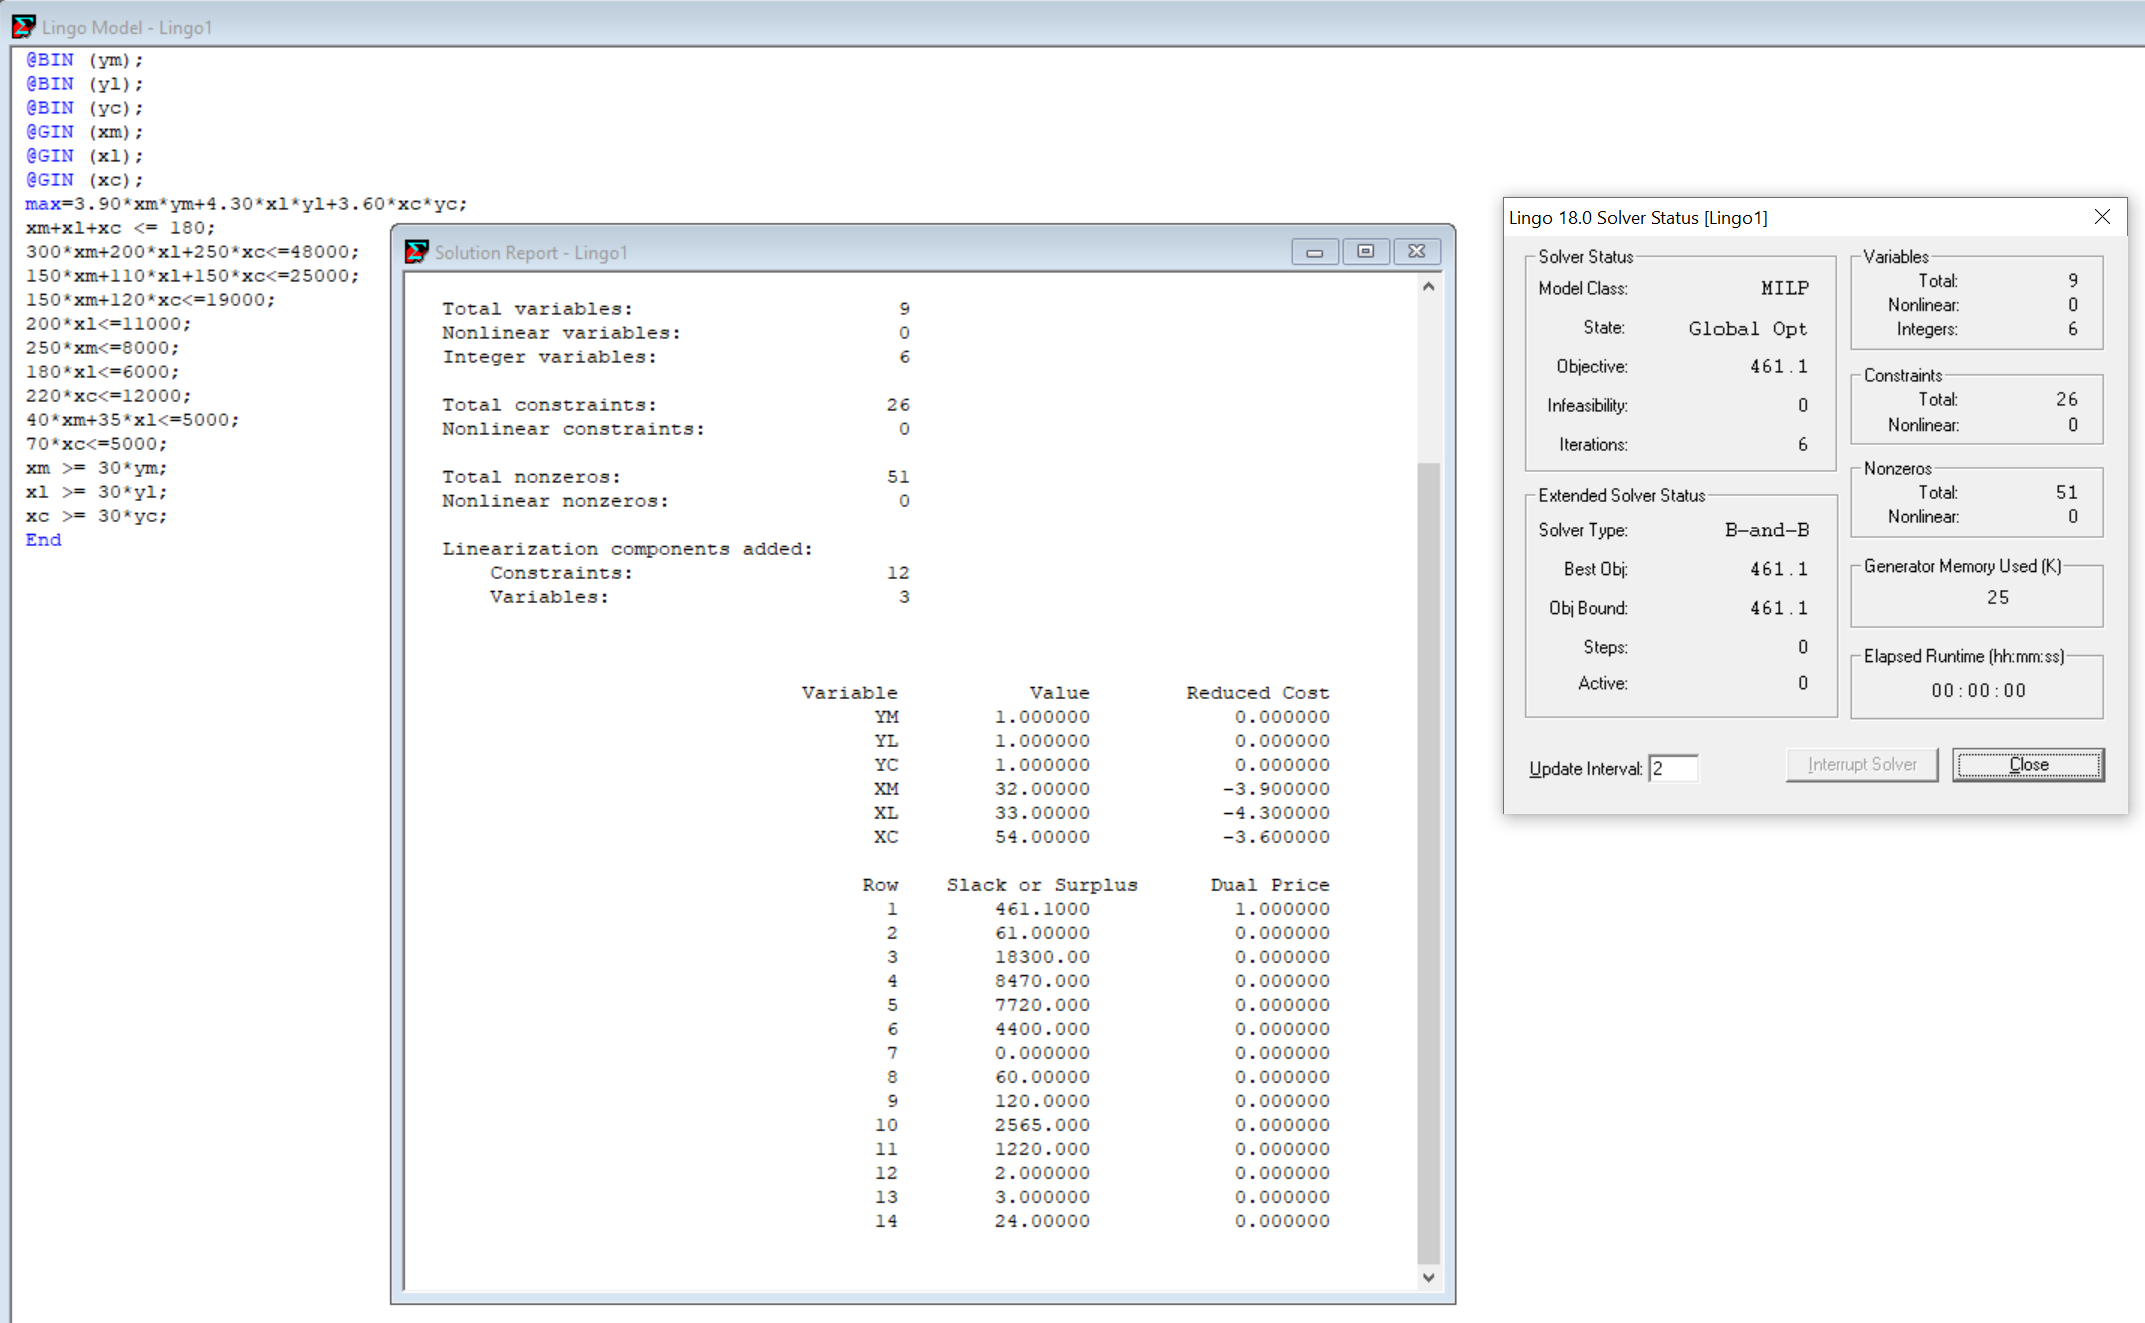
\includegraphics[width=1\linewidth]{src/ganzzahlig.png}
\end{centering}

$\to$ \textbf{Salatbar Optimalfall:} \\
- Jede Salatart wird angerichtet \\
- Salat M wird in 32 Portionen, Salat L in 33 Portionen und Salat C in 54 Portionen produziert

\end{document}